\subsection{Filtre inverse et stabilité}

\begin{frame}
\frametitle{Filtre inverse et stabilité}
	\footnotesize{\begin{align}
		H(z) &= \frac{
				(z-0.9\e^{j\pi/2})
				(z-0.9\e^{-j\pi/2})
				(z-0.95\e^{j\pi/8})
				(z-0.95\e^{-j\pi/8})
		  }{
				z(z+0.99)^2(z-0.8)
			} \\ \nonumber \\
		H^{-1}(z)  &= \frac{
				z(z+0.99)^2(z-0.8)
		  }{
				(z-0.9\e^{j\pi/2})
				(z-0.9\e^{-j\pi/2})
				(z-0.95\e^{j\pi/8})
				(z-0.95\e^{-j\pi/8})
			}
	\end{align}}
	% \begin{columns}[t] % Align columns at the top
	\begin{columns}
		\begin{column}{0.5\textwidth}
			\begin{table}
				\caption{Identités du filtre aberrant}
				\begin{tabular}{lll}
					\toprule
					Identité & Dans $H(Z)$ & Dans $H^{-1}(z)$ \\
					\midrule
					$0$                & $|\textrm{pôle}| <0$ & zéro \\
					$0.8$              & $|\textrm{pôle}| <0$ & zéro \\
					$-0.99$            & $|\textrm{pôle}| <0$ & zéro \\
					$0.9\e^{j\pi/2}$   & zéro & $|\textrm{pôle}| <0$ \\
					$0.9\e^{-j\pi/2}$  & zéro & $|\textrm{pôle}| <0$ \\
					$0.95\e^{j\pi/8}$  & zéro & $|\textrm{pôle}| <0$ \\
					$0.95\e^{-j\pi/8}$ & zéro & $|\textrm{pôle}| <0$ \\
					\bottomrule
				\end{tabular}
			\end{table}
		\end{column}
		\begin{column}{0.5\textwidth}
			\textbf{Réponse dans $\mathbb{R}$}: \\
			(pôles/zéros complexes ont leur conjugé) \\
			\begin{itemize}
				\item $0$ purement réel
				\item $0.8$ purement réel
				\item $-0.99$ purement réel\footnotemark[1]
				\item $0.9\e^{j\pi/2}\leftrightharpoons0.9\e^{-j\pi/2}$
				\item $0.95\e^{j\pi/8}\leftrightharpoons0.95\e^{-j\pi/8}$
			\end{itemize}
		\end{column}
	\end{columns}
		\footnotetext[1]{Puisque qu'il est élevé au carré, ce zéro est présent deux
		fois dans le filtre}
\end{frame}

\begin{frame}
\frametitle{Résultats}

	\begin{columns}[t]
		\begin{column}{0.32\textwidth}
			\begin{figure}
				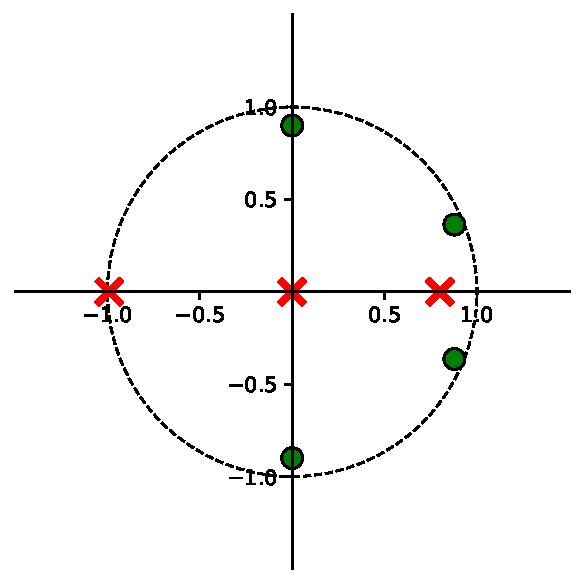
\includegraphics[width=1\linewidth]{figures/aberration-zplane-inv.pdf}
				\caption{\footnotesize{Filtre réparateur}}
			\end{figure}
		\end{column}

		\begin{column}{0.32\textwidth}
			\begin{figure}
				
\includegraphics[width=\linewidth]{figures/aberration-before.png}
				\caption{\footnotesize{Avec l'aberration}}
			\end{figure}
		\end{column}

		\begin{column}{0.32\textwidth}
			\begin{figure}
				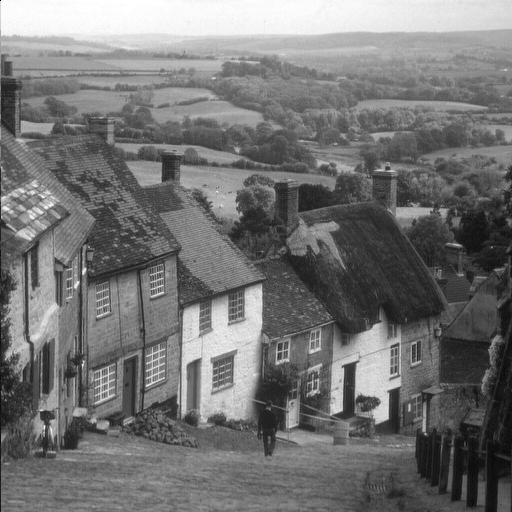
\includegraphics[width=\linewidth]{figures/aberration-after.png}
				\caption{\footnotesize{Aberration corrigée}}
			\end{figure}
		\end{column}
	\end{columns}

\end{frame}
